\documentclass[a4paper]{article}
\usepackage[a4paper,margin=0mm]{geometry}
\usepackage{fontspec}
\usepackage{unicode-math}
\usepackage{tikz}
\usetikzlibrary{calc}
\usepackage[table]{xcolor}
\usepackage[absolute]{textpos}
\usepackage{enumitem}
\usepackage{array}
\usepackage{multirow}

\setmainfont{Libertinus Serif}
\setsansfont{Libertinus Sans}
\setmathfont{Libertinus Math}

\definecolor{accent}{HTML}{0F6A52}
\definecolor{badge}{HTML}{A9CFC2}
\definecolor{ink}{HTML}{2A2E30}

\setlength{\TPHorizModule}{1mm}
\setlength{\TPVertModule}{1mm}
\setlength{\parindent}{0pt}
\pagestyle{empty}
\binoppenalty=10000 \relpenalty=10000

\newcommand{\LCOL}{16mm}
\newcommand{\RCOL}{111mm}
\newcommand{\COLW}{83mm}

\newcommand{\topicheader}[2]{%
\begin{textblock*}{194mm}(16mm,10mm)
\begin{tikzpicture}
\node[fill=accent,text=white,font=\sffamily\bfseries\fontsize{13}{13}\selectfont,
      minimum width=9mm,minimum height=9mm,inner sep=0pt] at (4.5mm,-4.5mm) {#1};
\node[font=\sffamily\bfseries\fontsize{15}{16}\selectfont,text=ink,anchor=west] at (12mm,-4.5mm) {#2};
\end{tikzpicture}
\end{textblock*}
\begin{textblock*}{194mm}(16mm,22.5mm)

\begin{tikzpicture}
\fill[accent] (0,0) rectangle (194mm,0.5mm);
\end{tikzpicture}
\end{textblock*}
}

\newcommand{\pagefooter}[1]{%
\begin{textblock*}{194mm}(8mm,286.41mm)
  
\begin{tikzpicture}
    \fill[accent] (0,0) rectangle (194mm,0.6mm);
  \end{tikzpicture}
\end{textblock*}
\begin{textblock*}{63.59mm}(8mm,288.27mm)
  {\sffamily\bfseries\color{accent}\fontsize{13}{16}\selectfont SAT 1200+}
\end{textblock*}
\begin{textblock*}{10mm}(188mm,288.27mm)
  \centering{\sffamily\color{accent}\fontsize{14}{16}\selectfont #1}
\end{textblock*}
}

\newcommand{\colrule}[2]{%
\begin{textblock*}{1mm}(105mm,#1mm)
\begin{tikzpicture}
\draw[black!65,line width=0.5pt] (0,0) -- (0,#2mm);
\end{tikzpicture}
\end{textblock*}
}

% Page kicker: left = module line, right = question range
\newcommand{\pagekicker}[2]{%
\begin{textblock*}{194mm}(16mm,25.2mm)
{\sffamily\bfseries\fontsize{10.5}{12}\selectfont\color{accent}#1}\hfill{\sffamily\fontsize{10}{12}\selectfont\color{black!70}#2}
\end{textblock*}
}

\setlength{\fboxsep}{1.4pt}
\setlength{\fboxrule}{0.5pt}
\newcommand{\pnum}[1]{\fcolorbox{ink}{white}{\sffamily\bfseries\fontsize{8}{8}\selectfont #1}~}

% centered display line inside a stem
\newcommand{\dsp}[1]{\par\vspace{1.4mm}\centerline{#1}\vspace{1.8mm}}

% student-produced response box
\newcommand{\gridbox}{%
\par\vspace{3mm}\noindent

\begin{tikzpicture}
\node[anchor=south west,font=\sffamily\bfseries\fontsize{7.5}{9}\selectfont,text=accent,inner sep=0pt] at (0,0.3mm) {STUDENT-PRODUCED RESPONSE};
\draw[ink,line width=0.7pt] (0,-9.5mm) rectangle (40mm,-0.8mm);
\node[anchor=west,font=\sffamily\fontsize{7.5}{9}\selectfont,text=black!55,inner sep=0pt] at (43mm,-5.2mm) {Write your answer in the box.};
\end{tikzpicture}\par}

\arrayrulecolor{accent}
\setlength{\arrayrulewidth}{0.7pt}
\renewcommand{\arraystretch}{1.35}

\newcommand{\figwrap}[1]{\par\vspace{2.5mm}\centerline{{\arrayrulecolor{ink}\setlength{\arrayrulewidth}{0.5pt}\renewcommand{\arraystretch}{1.3}#1}}\vspace{0.5mm}}


\setlength{\tabcolsep}{3pt}
\renewcommand{\arraystretch}{1.5}
\begin{document}

\topicheader{7}{Mock Test 7}
\pagefooter{1}
\mbox{}%

\begin{textblock*}{194mm}(16mm,28.5mm)
{\sffamily\bfseries\color{accent}\fontsize{17}{20}\selectfont Answer Sheet\par}
\vspace{0.6mm}
{\sffamily\color{ink}\fontsize{10}{12.5}\selectfont Check your answers after you finish both modules, then circle the tags of the questions you missed.\par}
\end{textblock*}

\begin{textblock*}{85mm}(16mm,46mm)
{\fontsize{10.5}{13}\selectfont
\begin{tabular}{|>{\centering\arraybackslash}p{9mm}|>{\centering\arraybackslash}p{20mm}|>{\centering\arraybackslash}p{19mm}|>{\centering\arraybackslash}p{13mm}|}
\hline
\rowcolor{accent}\multicolumn{4}{|c|}{\textcolor{white}{\textbf{Module 1}}}\\\hline
\rowcolor{badge!55}\textbf{Q} & \textbf{Answer} & \textbf{Domain} & \textbf{Level}\\\hline
1 & C & ALG & E\\\hline
2 & A & ADV & E\\\hline
3 & 300$^{\ast}$ & PSDA & E\\\hline
4 & D & GT & E\\\hline
5 & B & ALG & E\\\hline
6 & A & ADV & E\\\hline
7 & 5$^{\ast}$ & ALG & E\\\hline
8 & C & ADV & E\\\hline
9 & D & PSDA & M\\\hline
10 & B & ALG & M\\\hline
11 & 5$^{\ast}$ & ADV & M\\\hline
12 & C & GT & M\\\hline
13 & A & ALG & M\\\hline
14 & 4.35$^{\ast}$ & PSDA & M\\\hline
15 & D & ADV & M\\\hline
16 & B & ALG & M\\\hline
17 & C & ADV & M\\\hline
18 & 50$^{\ast}$ & ALG & M\\\hline
19 & A & ADV & M\\\hline
20 & D & ADV & H\\\hline
21 & 1260$^{\ast}$ & ALG & H\\\hline
22 & B & GT & H\\\hline
\end{tabular}}
\end{textblock*}

\begin{textblock*}{85mm}(110mm,46mm)
{\fontsize{10.5}{13}\selectfont
\begin{tabular}{|>{\centering\arraybackslash}p{9mm}|>{\centering\arraybackslash}p{20mm}|>{\centering\arraybackslash}p{19mm}|>{\centering\arraybackslash}p{13mm}|}
\hline
\rowcolor{accent}\multicolumn{4}{|c|}{\textcolor{white}{\textbf{Module 2} \;(harder route)}}\\\hline
\rowcolor{badge!55}\textbf{Q} & \textbf{Answer} & \textbf{Domain} & \textbf{Level}\\\hline
1 & B & ALG & E\\\hline
2 & D & ADV & E\\\hline
3 & A & PSDA & M\\\hline
4 & 10$^{\ast}$ & ALG & M\\\hline
5 & C & ADV & M\\\hline
6 & D & GT & M\\\hline
7 & A & ALG & M\\\hline
8 & 6$^{\ast}$ & ADV & M\\\hline
9 & B & PSDA & M\\\hline
10 & C & ALG & M\\\hline
11 & 12$^{\ast}$ & ADV & M\\\hline
12 & B & ALG & M\\\hline
13 & A & ADV & H\\\hline
14 & 44$^{\ast}$ & PSDA & H\\\hline
15 & D & ALG & H\\\hline
16 & C & ADV & H\\\hline
17 & B & GT & H\\\hline
18 & 35$^{\ast}$ & ADV & H\\\hline
19 & D & ALG & H\\\hline
20 & C & ALG & H\\\hline
21 & 24$^{\ast}$ & GT & H\\\hline
22 & A & ADV & H\\\hline
\end{tabular}}
\end{textblock*}

% ---- raw score box ----
\begin{textblock*}{178mm}(16mm,236mm)
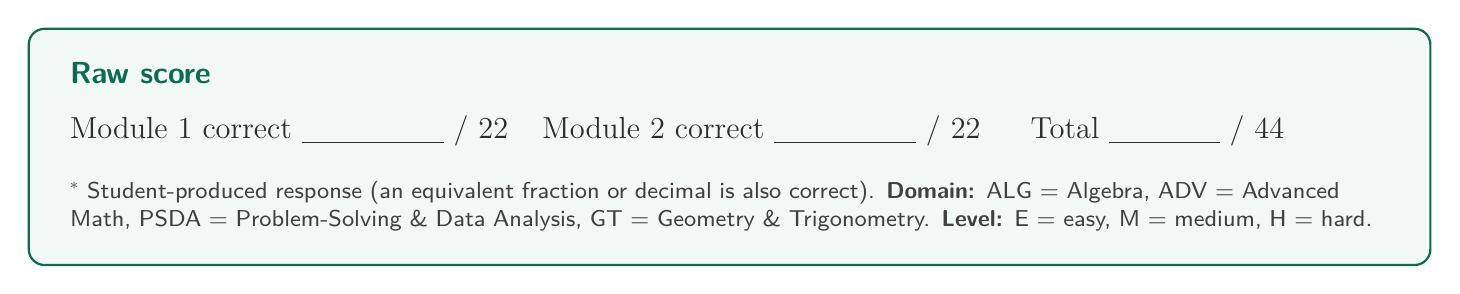
\begin{tikzpicture}
\draw[accent,line width=0.8pt,rounded corners=2mm,fill=badge!15] (0,0) rectangle (178mm,-30mm);
\node[anchor=north west,font=\sffamily\bfseries\fontsize{11}{13}\selectfont,text=accent] at (4mm,-3mm) {Raw score};
\node[anchor=west,font=\fontsize{11}{13}\selectfont,text=ink] at (4mm,-13mm) {Module 1 correct \rule[-0.6mm]{18mm}{0.5pt} / 22};
\node[anchor=west,font=\fontsize{11}{13}\selectfont,text=ink] at (64mm,-13mm) {Module 2 correct \rule[-0.6mm]{18mm}{0.5pt} / 22};
\node[anchor=west,font=\fontsize{11}{13}\selectfont,text=ink] at (126mm,-13mm) {Total \rule[-0.6mm]{14mm}{0.5pt} / 44};
\node[anchor=west,text width=170mm,font=\sffamily\fontsize{8.3}{10.2}\selectfont,text=black!75] at (4mm,-22.5mm)
 {$^{\ast}$ Student-produced response (an equivalent fraction or decimal is also correct). \textbf{Domain:} ALG = Algebra, ADV = Advanced Math, PSDA = Problem-Solving \& Data Analysis, GT = Geometry \& Trigonometry. \textbf{Level:} E = easy, M = medium, H = hard.};
\end{tikzpicture}
\end{textblock*}

\end{document}
